
\section{Análisis técnico}
Como se ha explicado en el capítulo~\ref{sec:terminos_basicos}, el \textbf{análisis técnico} (también llamado \textbf{charting}) es una forma de predecir los movimientos futuros de precios basándose únicamente en la observación del historial de precios (que también puede incluir volúmenes de tráfico). Por otro lado, el \textbf{análisis fundamental} se basa en factores subyacentes al instrumento financiero, como la salud de la empresa, el estado de la economía, etc. Esto puede incluir análisis económicos o políticos generales, o análisis de factores específicos de la acción (p.e.\ el calentamiento global en las nevadas en los Alpes, si se trata de una empresa de viajes).

En la práctica se usa una combinación de ambos tipos de análisis. Se considera que el análisis técnico es especialmente útil para predecir los movimientos del mercado; el análisis fundamental puede predecir la dirección correcta, pero no necesariamente cuándo ocurrirá el movimiento.



\begin{itemize}
    \item \textbf{Plotting}: Es el gráfico más simple. En ocasiones el eje vertical es logarítmico para para representar el retorno más que el valor absoluto de la acción. También hay veces que aparece un gráfico con el volumen de transacciones.
        \begin{figure}[H]
            \centering
            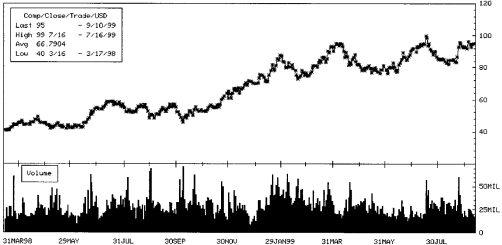
\includegraphics[width=0.65\linewidth]{Imagenes/Parte1/16_Prediccion/Plotting.png}
            \caption{Ejemplo de un gráfico de precios}
        \end{figure}
    \item \textbf{Resistance}: Es un nivel de precio que un activo parece tener dificultades para superar. Puede ser un valor máximo alcanzado previamente o una cifra (redonda) psicológicamente importante.
        \begin{figure}[H]
            \centering
            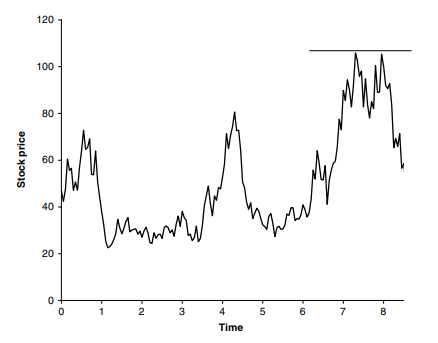
\includegraphics[width=0.65\linewidth]{Imagenes/Parte1/16_Prediccion/Resistance.png}
            \caption{Ejemplo de un nivel de resistencia}
        \end{figure}
    \item \textbf{Support}: Es un nivel por debajo del cual el precio de un activo parece reacio a caer. Puede haber suficiente demanda a este bajo precio para evitar que siga bajando.
        \begin{figure}[H]
            \centering
            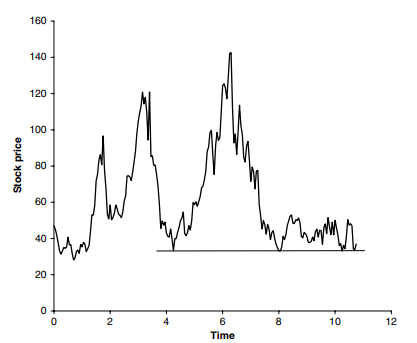
\includegraphics[width=0.65\linewidth]{Imagenes/Parte1/16_Prediccion/Support.png}
            \caption{Ejemplo de un nivel de soporte}
        \end{figure}
    \item \textbf{Trend lines}: son similares al soporte y la resistencia. Se forman uniendo picos y/o valles sucesivos en el historial de precios para formar un nivel de soporte o resistencia ascendente o descendente.
        \begin{figure}[H]
            \centering
            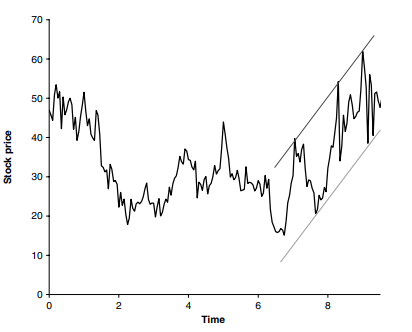
\includegraphics[width=0.65\linewidth]{Imagenes/Parte1/16_Prediccion/Trendlines.png}
            \caption{Ejemplo de una línea de tendencia}
        \end{figure}
    \item \textbf{Moving Averages}: se pueden calcular de varias maneras, con distintas ventanas temporales o incluso calcular medias ponderadas exponencialmente. Se supone que  destilan la tendencia básica de un precio suavizando el ruido aleatorio. Se suelen calcular dos medias: una a corto plazo y otra a largo plazo. Cuando la media a corto plazo cruza por encima de la de largo plazo, se considera una señal de compra; cuando cruza por debajo, es una señal de venta. 
    \item \textbf{Indice de fuerza relativa (RFI)}: es el porcentaje de movimientos alcistas en los últimos $N$ días. Un valor superior al 70 \% se considera sobrecomprado y, por lo tanto, es probable que baje, y un valor inferior al 30 \% se considera sobrevendido y debería subir.
    \item \textbf{Oscillators}: es otro indicador de condiciones de sobrecompra o sobreventa. Una forma de calcularlo es la siguiente. Se define $k$ como:
    \[
        k = 100 \times \frac{\text{Cierre actual} - \text{mínimo en } n \text{ periodos}}{\text{Máximo en } n \text{ periodos} - \text{mínimo en } n \text{ periodos}}
    \]
    Luego se toma un promedio móvil de los últimos tres días, por ejemplo. Este promedio se representa en el tiempo y cualquier movimiento fuera del rango 30--70\% podría indicar un movimiento en el activo.
        \begin{figure}[H]
            \centering
            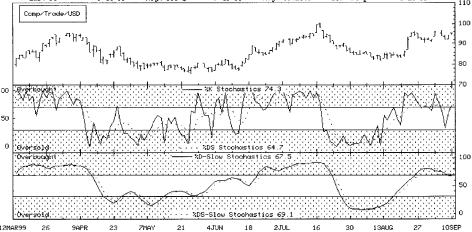
\includegraphics[width=0.65\linewidth]{Imagenes/Parte1/16_Prediccion/Oscillator.png}
            \caption{Ejemplo de un oscilador}
        \end{figure}
    \item \textbf{Bollinger Bands}: son gráficos de un número específico de desviaciones estándar por encima y por debajo de una media móvil específica. Se considera que el precio está sobrecomprado cuando toca la banda superior y sobrevendido cuando toca la banda inferior.
        \begin{figure}[H]
            \centering
            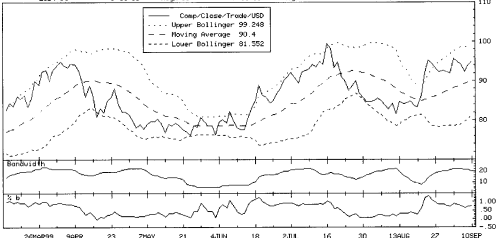
\includegraphics[width=0.65\linewidth]{Imagenes/Parte1/16_Prediccion/Bollinger Bands.png}
            \caption{Ejemplo de bandas de Bollinger}
        \end{figure}
    \item \textbf{Miscellaneous Patterns}: son patrones que se pueden encontrar en los gráficos. Es pseudociencia. Algunos patrones:
        \begin{itemize}
            \item \textbf{Head and shoulders}: Hay un hombro izquierdo y uno derecho con la cabeza elevándose por encima. A continuación del hombro derecho debería producirse una caída drástica en el precio del activo. Este patrón se considera uno de los predictores más fiables. También se observa en una formación invertida.
                \begin{figure}[H]
                    \centering
                    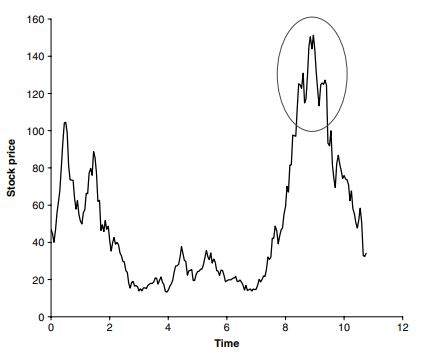
\includegraphics[width=0.65\linewidth]{Imagenes/Parte1/16_Prediccion/Head and shoulders.png}
                    \caption{Ejemplo de un patrón de cabeza y hombros}
                \end{figure}
            \item \textbf{Saucer tops and bottoms/ rounding tops and bottoms}: Son el resultado de un cambio gradual en la oferta y la demanda. Su forma suele ser bastante simétrica a medida que los precios suben y bajan. Estos patrones son bastante raros. No contienen información sobre la fuerza de la nueva tendencia.
                \begin{figure}[H]
                    \centering
                    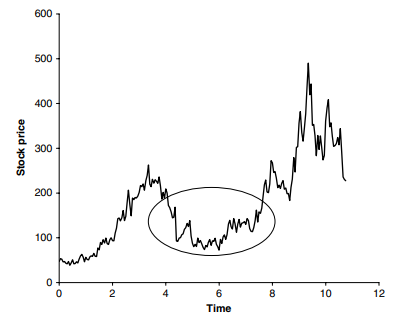
\includegraphics[width=0.65\linewidth]{Imagenes/Parte1/16_Prediccion/Saucer bottom.png}
                    \caption{Ejemplo de un patrón de plato}
                \end{figure}
            \item \textbf{Double and triple tops and bottoms}: Son patrones bastante raros, siendo el triple aún más raro que el doble. El doble techo se asemeja a una M y el doble suelo a una W. El triple techo es similar, pero con tres picos. La clave de los picos y valles es que todos deben estar aproximadamente al mismo nivel.
                \begin{figure}[H]
                    \centering
                    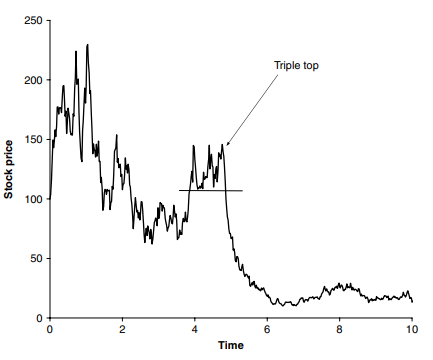
\includegraphics[width=0.65\linewidth]{Imagenes/Parte1/16_Prediccion/Triple top.png}
                    \caption{Ejemplo de un patrón de triple techo}
                \end{figure}
        \end{itemize}
    \item \textbf{Japanese Candlesticks}: Registran los precios de apertura y cierre, así como los máximos y mínimos del día. Se dibuja un rectángulo que se extiende desde el cierre hasta la apertura, y se colorea de blanco si el cierre está por encima de la apertura y de negro si está por debajo de la apertura. El rango máximo-mínimo se marca con una línea continua. Ciertas combinaciones de velas, que aparecen consecutivamente, tienen significados y nombres especiales, como ``Hombre Colgado'' y ``Dos Cuervos con Brecha alcista''. Véase Figura~\ref{fig:meanings_candlesticks} para ver las velas en acción. En este gráfico de letras se muestran: ``HR'' = Harami Bajista, ``D'' = Doji (que representa indecisión), ``BH'' = Harami Alcista, ``EL'' = Línea Envolvente Bajista y ``H'' = Hombre Colgado (que representa un cambio de tendencia).
        \begin{figure}[H]
            \centering
            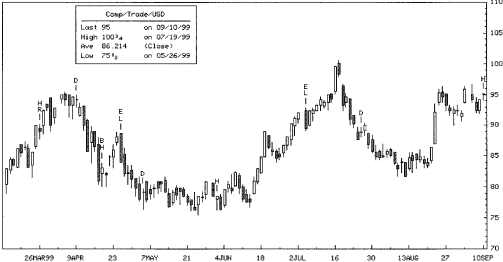
\includegraphics[width=0.65\linewidth]{Imagenes/Parte1/16_Prediccion/Candlestick char.png}
            \caption{Ejemplo de un gráfico de velas japonesas}
        \end{figure}
        \begin{figure}[H]
            \centering
            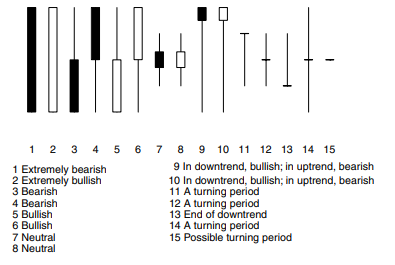
\includegraphics[width=0.65\linewidth]{Imagenes/Parte1/16_Prediccion/Meanings candlesticks.png}
            \caption{Significado de algunas velas japonesas}
            \label{fig:meanings_candlesticks}
        \end{figure}
    \item \textbf{Point and Figure Charts}: No tienen una escala temporal explícita en el eje horizontal. Cada casilla del gráfico representa un movimiento predefinido del precio de un activo. Las casillas permiten discretizar los movimientos del precio de los activos, en lugar de hacerlo en el tiempo. Por cada subida consecutiva del precio de un activo del tamaño de la casilla, dibuje una ``X'' en la casilla, en una columna ascendente, una encima de la otra. Cuando esta tendencia alcista termine y el activo baje, comience a escribir una ``O'' en una columna descendente, a la derecha de las X ascendentes anteriores.
        \begin{itemize}
            \item Una columna larga de X indica que la demanda supera a la oferta.
            \item Una columna larga de O indica que la oferta supera a la demanda.
            \item Columnas cortas ascendentes y descendentes indican un equilibrio entre oferta y demanda.
        \end{itemize}
        \begin{figure}[H]
            \centering
            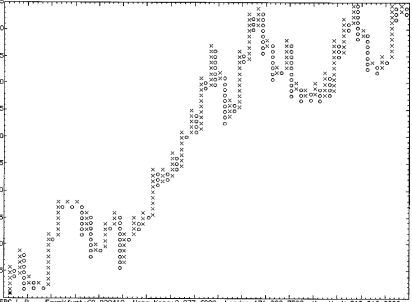
\includegraphics[width=0.65\linewidth]{Imagenes/Parte1/16_Prediccion/Point Figure Chart.png}
            \caption{Ejemplo de un gráfico de Puntos y Figuras}
        \end{figure}
    \item \textbf{Volume}: El número de contratos negociados en un período determinado. Un precio al alza y un volumen alto indican un mercado con una tendencia alcista sólida. Sin embargo, un precio al alza con un volumen bajo podría indicar que el mercado está a punto de cambiar de rumbo.
    \item \textbf{Open interest}: El número de contratos de futuros aún vigentes, aquellos que no se han liquidado. Dado que hay el mismo número de compradores y vendedores, el open interest no proporciona necesariamente información direccional, pero un aumento en el open interest puede indicar que una tendencia existente es fuerte.
\end{itemize}





\section{Wave theory}
Existen algunas teorías de predicción de precios basadas en ciclos o olas del mercado.

\subsection{Olas de Elliott y números de Fibonacci}
Alpha N. Elliott observó patrones, ondas o ciclos repetitivos en los precios. En términos generales, se supone que hay cinco puntos en una onda alcista y tres en una bajista (véase la Figura 20.14). Dentro de esta teoría de ondas de Elliott también se supone que existe cierta capacidad predictiva en cuanto al tamaño de los picos de cada onda. Además, se supone que la proporción de picos en una tendencia es bastante constante; la proporción entre el segundo pico y el primero debería ser de aproximadamente 1,618 y entre el tercero y el segundo, de 2,618. El valor 1,618 se acerca bastante a Golden ratio $\frac{1}{2}(\sqrt{5}+1)$; y es el ratio en números consecutivos de Fibonacci dados por $a_n = a_{n-1}+a_{n-2}$ para un $n$ grande.
\begin{figure}[H]
    \centering
    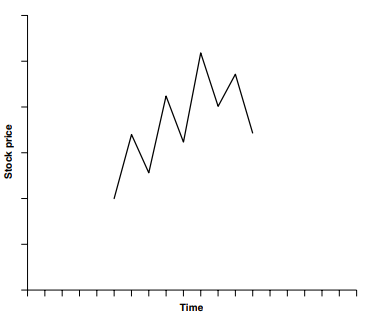
\includegraphics[width=0.65\linewidth]{Imagenes/Parte1/16_Prediccion/Elliot waves.png}
    \caption{Ejemplo de ondas de Elliott}
\end{figure}



También hay otras hipótesis como la de Gann Charts.





